\begin{center}

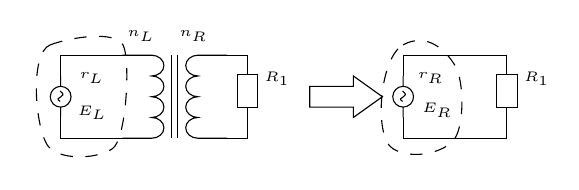
\begin{tikzpicture}[x=0.75pt,y=0.75pt,yscale=-1,xscale=1]
%uncomment if require: \path (0,300); %set diagram left start at 0, and has height of 300

%Shape: Inductor [id:dp27353243461904087] 
\draw   (174.75,120) -- (188.87,120) .. controls (192.11,120) and (194.75,122.24) .. (194.75,125) .. controls (194.75,127.76) and (192.11,130) .. (188.87,130) .. controls (192.11,130) and (194.75,132.24) .. (194.75,135) .. controls (194.75,137.76) and (192.11,140) .. (188.87,140) .. controls (192.11,140) and (194.75,142.24) .. (194.75,145) .. controls (194.75,147.76) and (192.11,150) .. (188.87,150) .. controls (192.11,150) and (194.75,152.24) .. (194.75,155) .. controls (194.75,157.76) and (192.11,160) .. (188.87,160) -- (174.75,160) ;
%Shape: Inductor [id:dp5366739264171354] 
\draw   (225.25,160) -- (211.13,160) .. controls (207.89,160) and (205.25,157.76) .. (205.25,155) .. controls (205.25,152.24) and (207.89,150) .. (211.13,150) .. controls (207.89,150) and (205.25,147.76) .. (205.25,145) .. controls (205.25,142.24) and (207.89,140) .. (211.13,140) .. controls (207.89,140) and (205.25,137.76) .. (205.25,135) .. controls (205.25,132.24) and (207.89,130) .. (211.13,130) .. controls (207.89,130) and (205.25,127.76) .. (205.25,125) .. controls (205.25,122.24) and (207.89,120) .. (211.13,120) -- (225.25,120) ;
%Straight Lines [id:da43269268551005813] 
\draw    (201.5,120) -- (201.5,160)(198.5,120) -- (198.5,160) ;
%Shape: Resistor [id:dp1038795254331022] 
\draw   (240,129.46) -- (240,145.29) -- (230,145.29) -- (230,129.46) -- (240,129.46) -- cycle (235,125) -- (235,129.46) (235,145.29) -- (235,149.75) ;
%Straight Lines [id:da6753753426347646] 
\draw    (225,120) -- (235,120) -- (235,125) ;
%Straight Lines [id:da7303120384870547] 
\draw    (225.25,160) -- (235,160) -- (235,149.75) ;
%Straight Lines [id:da43936866820960474] 
\draw    (145,150) -- (145,160) -- (175,160) ;
%Straight Lines [id:da690920244145504] 
\draw    (145,130) -- (145,120) -- (175,120) ;
%Left Arrow [id:dp8411203729282917] 
\draw   (300,140) -- (286,150) -- (286,145) -- (265,145) -- (265,135) -- (286,135) -- (286,130) -- cycle ;
%Shape: Polygon Curved [id:ds39327187302490896] 
\draw  [dash pattern={on 4.5pt off 4.5pt}] (140,115) .. controls (150.63,111.08) and (171.25,108.17) .. (175,115) .. controls (178.75,121.83) and (176.75,160.33) .. (170,165) .. controls (163.25,169.67) and (147.13,170.88) .. (140,165) .. controls (132.87,159.12) and (129.37,118.92) .. (140,115) -- cycle ;
%Straight Lines [id:da07750105951735708] 
\draw    (310,150) -- (310,160) -- (349.75,160) ;
%Straight Lines [id:da012940209870557107] 
\draw    (310,130) -- (310,120) -- (350,120) ;
%Shape: Resistor [id:dp3053611810905341] 
\draw   (365,129.45) -- (365,145.3) -- (355,145.3) -- (355,129.45) -- (365,129.45) -- cycle (360,125) -- (360,129.45) (360,145.3) -- (360,149.75) ;
%Straight Lines [id:da2926170106984707] 
\draw    (349.75,120) -- (360,120) -- (360,125) ;
%Straight Lines [id:da6676712847117272] 
\draw    (349.75,160) -- (360,160) -- (360,149.75) ;
%Shape: Polygon Curved [id:ds5017644089146096] 
\draw  [dash pattern={on 4.5pt off 4.5pt}] (310,115) .. controls (321.38,108.83) and (330.5,117.42) .. (335,125) .. controls (339.5,132.58) and (339.37,153.17) .. (335,160) .. controls (330.63,166.83) and (314.38,170.83) .. (305,165) .. controls (295.62,159.17) and (298.62,121.17) .. (310,115) -- cycle ;
%Shape: Output [id:dp9397863536393916] 
\draw   (145,135) .. controls (147.76,135) and (150,137.24) .. (150,140) .. controls (150,142.76) and (147.76,145) .. (145,145) .. controls (142.24,145) and (140,142.76) .. (140,140) .. controls (140,137.24) and (142.24,135) .. (145,135) -- cycle (145,130) -- (145,135) (145,150) -- (145,145) ;
%Curve Lines [id:da553613385459726] 
\draw    (144.75,137.25) .. controls (149.17,140.5) and (140.92,140) .. (144.75,142.25) ;

%Shape: Output [id:dp721029072764221] 
\draw   (310,135) .. controls (312.76,135) and (315,137.24) .. (315,140) .. controls (315,142.76) and (312.76,145) .. (310,145) .. controls (307.24,145) and (305,142.76) .. (305,140) .. controls (305,137.24) and (307.24,135) .. (310,135) -- cycle (310,130) -- (310,135) (310,150) -- (310,145) ;
%Curve Lines [id:da018977894649552907] 
\draw    (309.75,137.25) .. controls (314.17,140.5) and (305.92,140) .. (309.75,142.25) ;


% Text Node
\draw (176,107) node [anchor=north west][inner sep=0.75pt]  [font=\tiny] [align=left] {$\displaystyle n_{L}$};
% Text Node
\draw (201,107) node [anchor=north west][inner sep=0.75pt]  [font=\tiny] [align=left] {$\displaystyle n_{R}$};
% Text Node
\draw (242,127) node [anchor=north west][inner sep=0.75pt]  [font=\tiny] [align=left] {$\displaystyle R_{1}$};
% Text Node
\draw (367,127) node [anchor=north west][inner sep=0.75pt]  [font=\tiny] [align=left] {$\displaystyle R_{1}$};
% Text Node
\draw (152,143) node [anchor=north west][inner sep=0.75pt]  [font=\tiny] [align=left] {$\displaystyle \ms E_{L}$};
% Text Node
\draw (316,127) node [anchor=north west][inner sep=0.75pt]  [font=\tiny] [align=left] {$\displaystyle r_{R}$};
% Text Node
\draw (153,127) node [anchor=north west][inner sep=0.75pt]  [font=\tiny] [align=left] {$\displaystyle r_{L}$};
% Text Node
\draw (318,142) node [anchor=north west][inner sep=0.75pt]  [font=\tiny] [align=left] {$\displaystyle \ms E_{R}$};

\end{tikzpicture}

\end{center}